\documentclass[12pt, a4paper]{article}
\usepackage[utf8]{inputenc}
\usepackage{physics}
\usepackage{graphicx}
\usepackage{amsmath}
\usepackage{cancel}
%code color
\usepackage{listings}
\usepackage{xcolor}

\definecolor{codegreen}{rgb}{0,0.6,0}
\definecolor{codegray}{rgb}{0.5,0.5,0.5}
\definecolor{codepurple}{rgb}{0.58,0,0.82}
\definecolor{backcolour}{rgb}{0.95,0.95,0.92}

\lstdefinestyle{mystyle}{
	backgroundcolor=\color{backcolour},   
	commentstyle=\color{codegreen},
	keywordstyle=\color{magenta},
	numberstyle=\tiny\color{codegray},
	stringstyle=\color{codepurple},
	basicstyle=\ttfamily\footnotesize,
	breakatwhitespace=false,         
	breaklines=true,                 
	captionpos=b,                    
	keepspaces=true,                 
	numbers=left,                    
	numbersep=5pt,                  
	showspaces=false,                
	showstringspaces=false,
	showtabs=false,                  
	tabsize=2
}

\lstset{style=mystyle}

\begin{document}
	\begin{center}
		Test 2   Superdense Coding
	\end{center}
	
	Mr. Phiphat Chomchit 630631028
	\begin{enumerate}
	\item This homework needs your understanding of basis change/rotation in linear algebra. The application is to use a qubit to encode classical bits. Initially, Alice and Bob share an EPR pair and there is a quantum channel from Alice to Bob. Alice wants to send classical bits to Bob. Superdense coding is a protocol where Alice sends one qubit to Bob, but the amount of transmitted information is two classical bits. This is done as follows.\\
	
	Alice has two classical bits, $b_1$ and $b_2$, and Alice shares an EPR pair with Bob. Recall that the EPR pair is
	
	$$\frac{1}{\sqrt{2}}\ket{00} + \frac{1}{\sqrt{2}}\ket{11}$$
	
	
	We assume that the first qubit belongs to Alice and the second Bob. Depending on which pair of classical bits Alice wants to send, the operations are as follows.\\
	
		\begin{center}
			\begin{tabular}{ |c|c|c|}
				\hline
				$b_1b_2$ & Alice’s Operation & State after Alice’s Operation \\
				\hline
				$00$ & Nothing & $\frac{1}{\sqrt{2}}\ket{00} + \frac{1}{\sqrt{2}}\ket{11}$\\
				\hline
				$01$ & X gate & $\frac{1}{\sqrt{2}}\ket{10} + \frac{1}{\sqrt{2}}\ket{01}$\\
				\hline
				$10$ & Z gate & $\frac{1}{\sqrt{2}}\ket{00} - \frac{1}{\sqrt{2}}\ket{11}$\\
				\hline
				$11$ & XZ gate & $\frac{1}{\sqrt{2}}\ket{10} - \frac{1}{\sqrt{2}}\ket{01}$\\
				\hline

			\end{tabular}
		\end{center}
		

	Now Alice passes her qubit through the quantum channel to Bob. Now Bob has access to both qubits and 
	applies CNOT gate to the first (control) and second (target) qubits, then applies H gate to the first qubit, 
	and lastly measures both qubits to obtain the classical bits Alice wants to send.
	
	Your job is to implement this superdense coding quantum circuit and demonstrates it works for each case 
	of 2 classical bits.
	
	\end{enumerate}
\newpage
	Ans.
	\begin{enumerate}
		\item Nothing
		\centering
			\begin{lstlisting}[language=Python, caption= Superdense Coding (Nothing)]
			OPENQASM 2.0;
			include "qelib1.inc";
			//initial qubits
			qreg q[2];
			creg c[2];
			
			//entangle state
			h q[0];
			cx q[0],q[1];
			
			//encoding
			id q[0];
			
			//decoding
			cx q[0],q[1];
			h q[0];
			measure q[0] -> c[0];
			measure q[1] -> c[1];
		\end{lstlisting}

			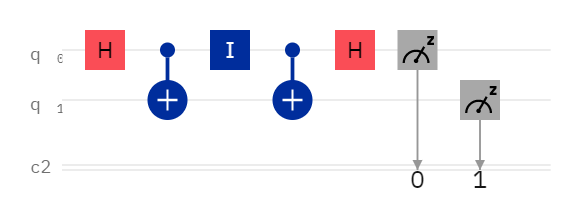
\includegraphics[scale=0.5]{circuit-i.png}
			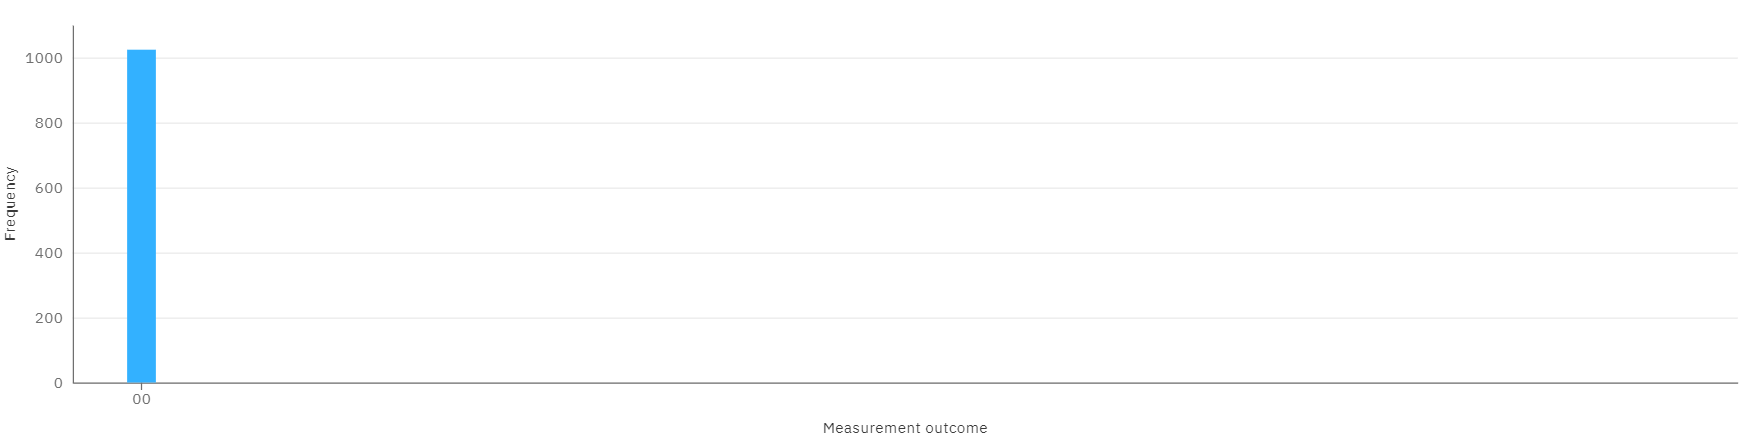
\includegraphics[scale=0.3]{bar-i.png}
			
		\newpage	
		\item X gate
		
					\begin{lstlisting}[language=Python, caption= Superdense Coding (X-gate)]
			OPENQASM 2.0;
			include "qelib1.inc";
			//initial qubits
			qreg q[2];
			creg c[2];
			
			//entangle state
			h q[0];
			cx q[0],q[1];
			
			//encoding
			x q[0];
			
			//decoding
			cx q[0],q[1];
			h q[0];
			measure q[0] -> c[0];
			measure q[1] -> c[1];
		\end{lstlisting}
	
		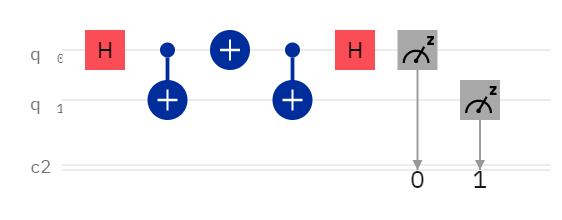
\includegraphics[scale=0.5]{circuit-x.png}
		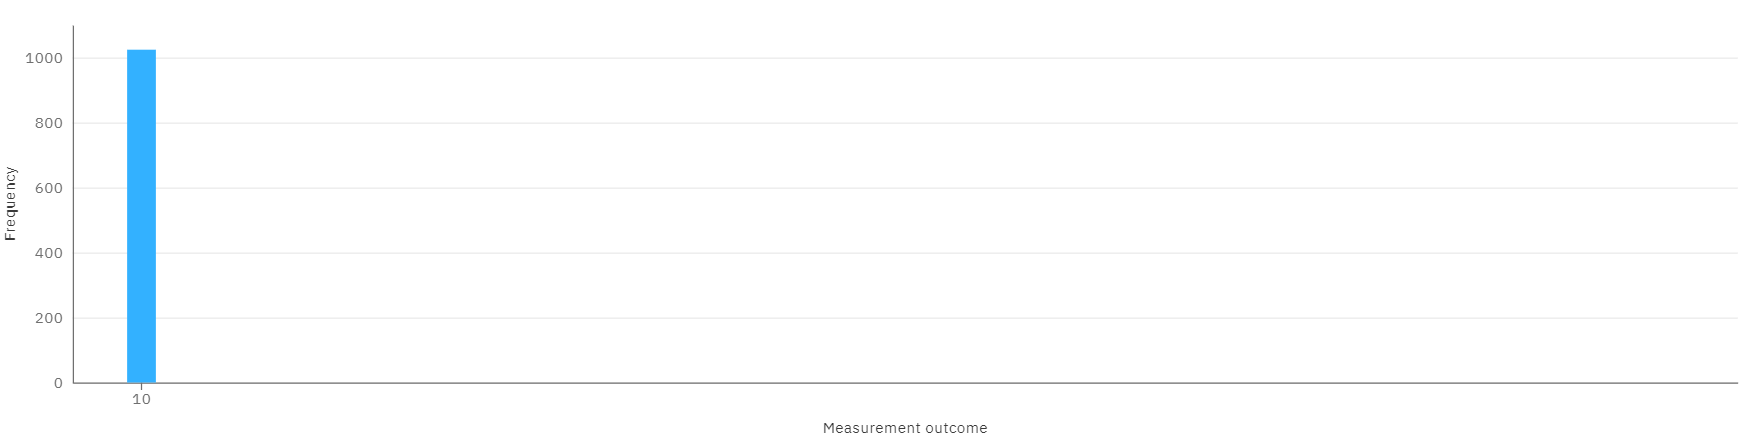
\includegraphics[scale=0.3]{bar-x.png}
		
		\newpage
		\item Z gate
		
		\begin{lstlisting}[language=Python, caption= Superdense Coding (Z-gate)]
			OPENQASM 2.0;
			include "qelib1.inc";
			//initial qubits
			qreg q[2];
			creg c[2];
			
			//entangle state
			h q[0];
			cx q[0],q[1];
			
			//encoding
			z q[0];
			
			//decoding
			cx q[0],q[1];
			h q[0];
			measure q[0] -> c[0];
			measure q[1] -> c[1];
		\end{lstlisting}
		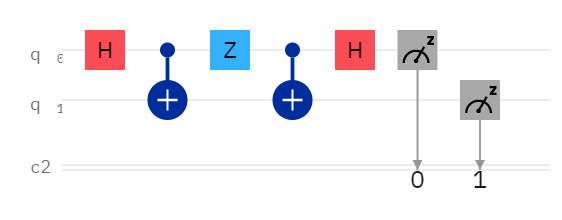
\includegraphics[scale=0.5]{circuit-z.png}
		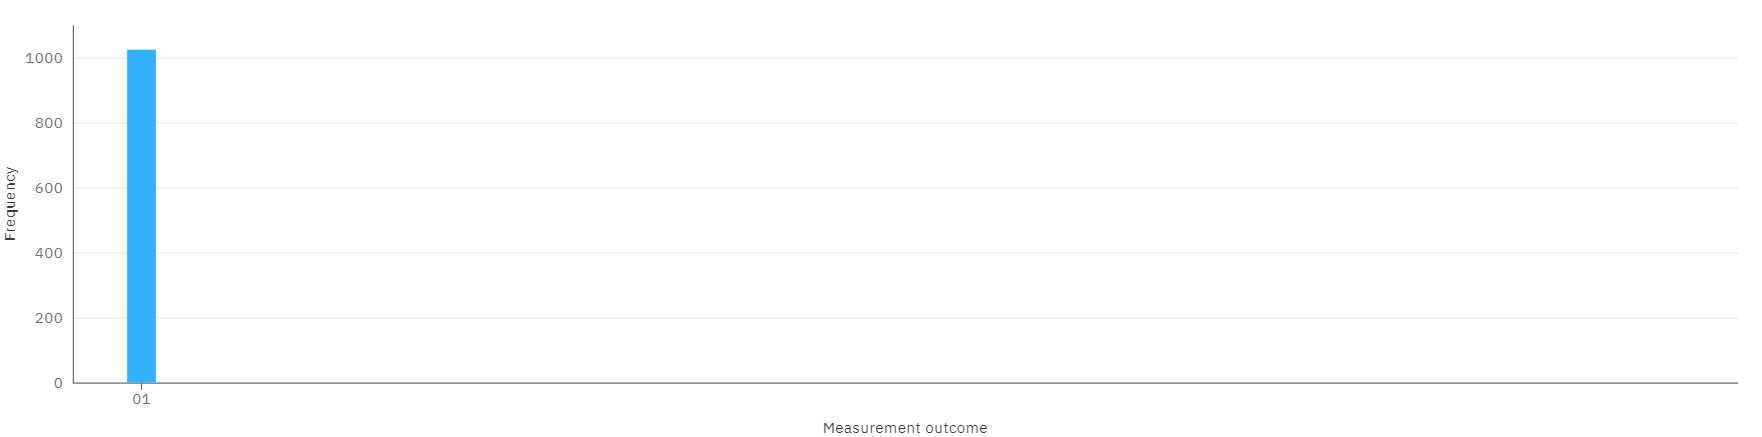
\includegraphics[scale=0.3]{bar-z.png}
		
		\newpage
		\item XZ gate
		
		\begin{lstlisting}[language=Python, caption= Superdense Coding (XZ-gate)]
			OPENQASM 2.0;
			include "qelib1.inc";
			//initial qubits
			qreg q[2];
			creg c[2];
			
			//entangle state
			h q[0];
			cx q[0],q[1];
			
			//encoding
			x q[0];
			z q[0];
			
			//decoding
			cx q[0],q[1];
			h q[0];
			measure q[0] -> c[0];
			measure q[1] -> c[1];
		\end{lstlisting}
		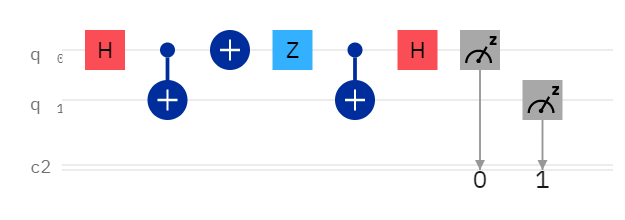
\includegraphics[scale=0.5]{circuit-xz.png}
		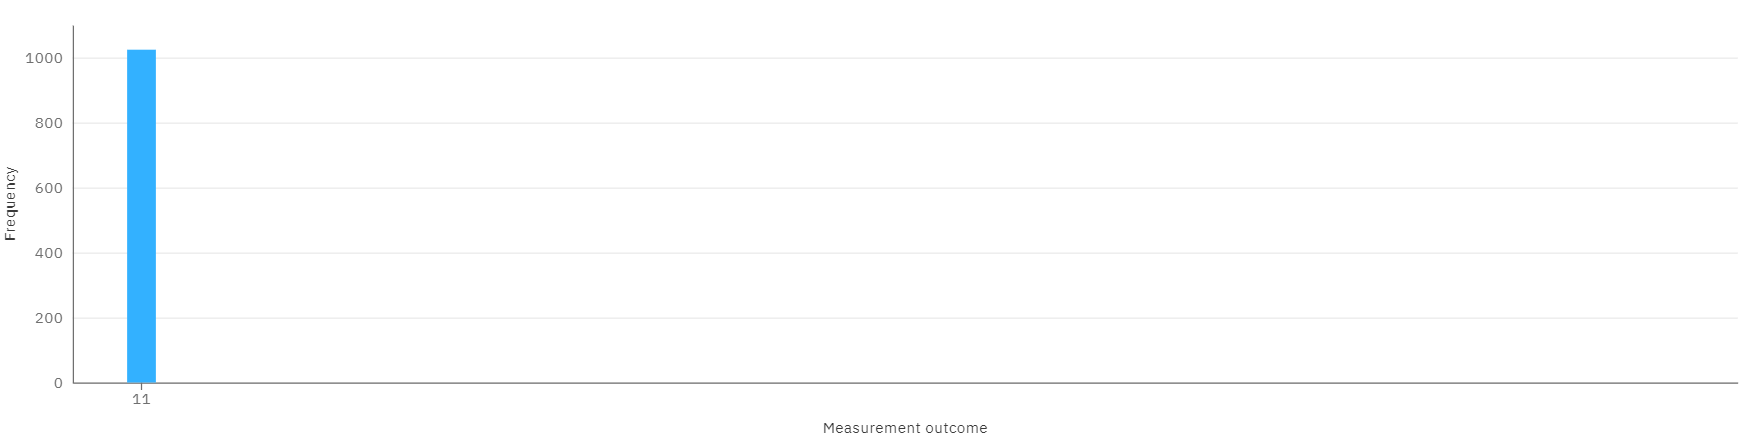
\includegraphics[scale=0.3]{bar-xz.png}
	\end{enumerate}
\end{document}